\documentclass[french]{article}

% Packages for french documents
\usepackage{babel}
\usepackage[utf8]{inputenc}
\usepackage[T1]{fontenc}

% Define some colors
\usepackage{color}
\definecolor{string}{RGB}{100, 200, 0}
\definecolor{comment}{RGB}{150, 150, 150}
\definecolor{identifier}{RGB}{100, 100, 200}

% Source code style
\usepackage{listings}
\lstset{
	basicstyle=\footnotesize\ttfamily, % sets font style for the code
	frame=single,                 % adds a frame around the code
	showstringspaces=false,       % underline spaces within strings
	tabsize=4,                    % sets default tabsize to 2 spaces
	breaklines=true,              % sets automatic line breaking
	breakatwhitespace=true,       % sets if automatic breaks should only happen at whitespace
	keywordstyle=\color{magenta}, % sets color for keywords
	stringstyle=\color{string},   % sets color for strings
	commentstyle=\color{comment}, % sets color for comments
	emphstyle=\color{identifier}, % sets color for comments
}

% Hyperlinks
\usepackage[hyphens]{url}
\usepackage[hidelinks]{hyperref}

% Graphics
\usepackage{graphicx}
\graphicspath{ {../img/} }

\title{Projet ARA : Paxos}
\date{Février 2021}
\author{Sylvain Joube, Nicolas Peugnet}

\begin{document}

\maketitle

\tableofcontents

\section*{Introduction}

Le but de ce projet est de d'étudier l'efficacité de l'algorithme de Paxos en faisant varier un certain nombre de paramètres.
La première chose à faire a été de coder l'algorithme à l'aide d'un simulateur afin de pouvoir lancer plusieurs expérimentations.
Nous avons utilisé PPI\footnote{\url{https://github.com/PolyProcessInterface/ppi}} pour cette tâche,
car cette API permet de lancer le code soit sur le simulateur Peersim soit via MPI et parce que réutiliser un projet réalisé par le passé était plus motivant pour au moins l'un de nous deux.
Ce n'était, comme on pouvait s'en douter, pas une si bonne idée que ça.

\section{Étude expérimentale 1}

Le but de cette première étude expérimentale est d'évaluer l'efficacité d'une unique itération de l'algorithme.
Les valeurs prises en compte pour quantifier cette efficacité sont :

\begin{enumerate}
	\item Le \textbf{temps de convergence} : le temps nécessaire au protocole pour que tous les nœuds reconnaissent le même leader.
	\item Le \textbf{nombre de rounds} nécessaires pour atteindre une majorité, c’est-à-dire pour que le consensus soit atteint.
	\item Le \textbf{nombre de messages} émis.
\end{enumerate}

Et les paramètres en fonctions desquels on veut évaluer ces critères sont :

\begin{enumerate}
	\item Le \textbf{nombre de nœuds} dans le système.
	\item L'\textbf{activation/désactivation} et \textbf{valeur d'incrément d’un temps de \emph{backoff}}.
	\item La \textbf{valeur du round initial} :
	\begin{itemize}
		\item Une version avec la valeur 0 (Paxos original).
		\item Une version avec l’identifiant du nœud.
	\end{itemize}
\end{enumerate}

En ce qui concerne la valeur d'incrément du temps de \emph{backoff} nous avons choisi d'utiliser le code suivant :

\begin{lstlisting}[language=java]
public int backoffDelay() {
	return (backoff + CommonState.r.nextInt(backoff)) * coef * retry;
}
\end{lstlisting}

Bien que ne permettant pas de faire d'autres courbes que des droites, cette méthode permet de tester différentes valeurs d'incrément ainsi que l'activation et désactivation du temps de \emph{backoff} à l'aide des deux paramètres \lstinline{backoff} et \lstinline{coef}.
Un nombre aléatoire est ajouté à ce délai afin d'éviter que tous les nœuds n'utilisent des valeurs trop proches l'une de l'autre à chaque nouvel essai.


%%%%%%%%%%%%%%%%%%%%%%%%%%%%%%%%%%%%%%%%%%%%%%%%%%%%
%%%%%%%% Ici il faut des joulis graphiques %%%%%%%%%
%%%%%%%%%%%%%%%%%%%%%%%%%%%%%%%%%%%%%%%%%%%%%%%%%%%%

On remarque que comme prévu, l'utilisation de l'identifiant du nœud comme valeur de round initial donne plus de chances aux nœuds ayant un grand identifiant.
Cette propriété permet donc d'arriver plus rapidement à un consensus et avec beaucoup moins d'envois de messages.





\section{Étude expérimentale 2 : Multi-Paxos séquentiel}

Cette étude n'a malheureusement pas pu être menée à terme.
Un début de code a été produit mais n'assurant pas les propriétés de sureté, il n'a pas été possible de l'utiliser à des fins d'expérimentations.

\section{Étude expérimentale 3 : Réduire le coût en messages}

Une fois encore, nous n'avons pas eu la possibilité de réaliser cette étude, car nous n'avons pas produit de code fonctionnel.
Cependant une idée a été retenue.

\section*{Conclusion}

\begin{quotation}
	"Rien ne sert de courir ; il faut partir à point."

	--- \emph{Jean de la Fontaine}
\end{quotation}









%%%%%%%%%%%%%%%%%%%%%%%%%%%%%%%%%%% Tout ce bloc est une démo à retirer plus tard %%%%%%%%%%%%%%%%%%%%%%%%%%%%%%%%%%%%%%%%%%%%%%%%
\section{Démo \LaTeX}

Dans la Figure \ref{fig:test} on remarque que l'humeur de Nicolas est fortement variable en fonction du temps.

\begin{figure}[ht]
    \centering
    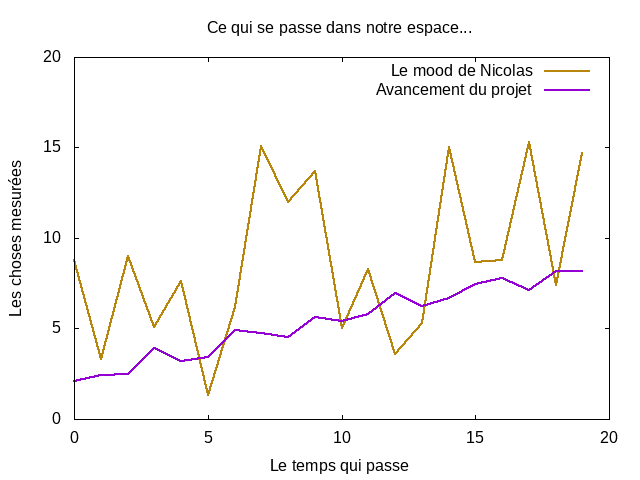
\includegraphics[width=1\textwidth]{test}
    \caption{Un joli graphique}
    \label{fig:test}
\end{figure}

%%%%%%%%%%%%%%%%%%%%%%%%%%%%%%%%%%% Fin du bloc de démo à retirer plus tard %%%%%%%%%%%%%%%%%%%%%%%%%%%%%%%%%%%%%%%%%%%%%%%%






\end{document}
